% Appendix details for MNIST-Rows sequence prediction experiments
\subsection{MNIST-Rows sequence prediction: additional details}\label{app:rnn-details}

This appendix complements Section~\ref{sec:mnist_rows_rnn} with additional qualitative rollout plots.


\paragraph{Autoregressive rollouts.}
We additionally include multi-step autoregressive row-completion rollouts to visually show next-element predictions of the two models. For each sample, the model is conditioned on 8, 16, or 24 of the image's first rows and predicts the next 4 rows; the remaining rows are shown as ground truth. The first red marker indicates the context-to-generation boundary, and the second red marker indicates the generation-to-ground-truth boundary. These rollouts are included for visual inspection, and long-horizon stability is not optimized in this study and rollout quality is not treated as a primary evaluation metric.


\begin{figure}[!ht]
  \centering
  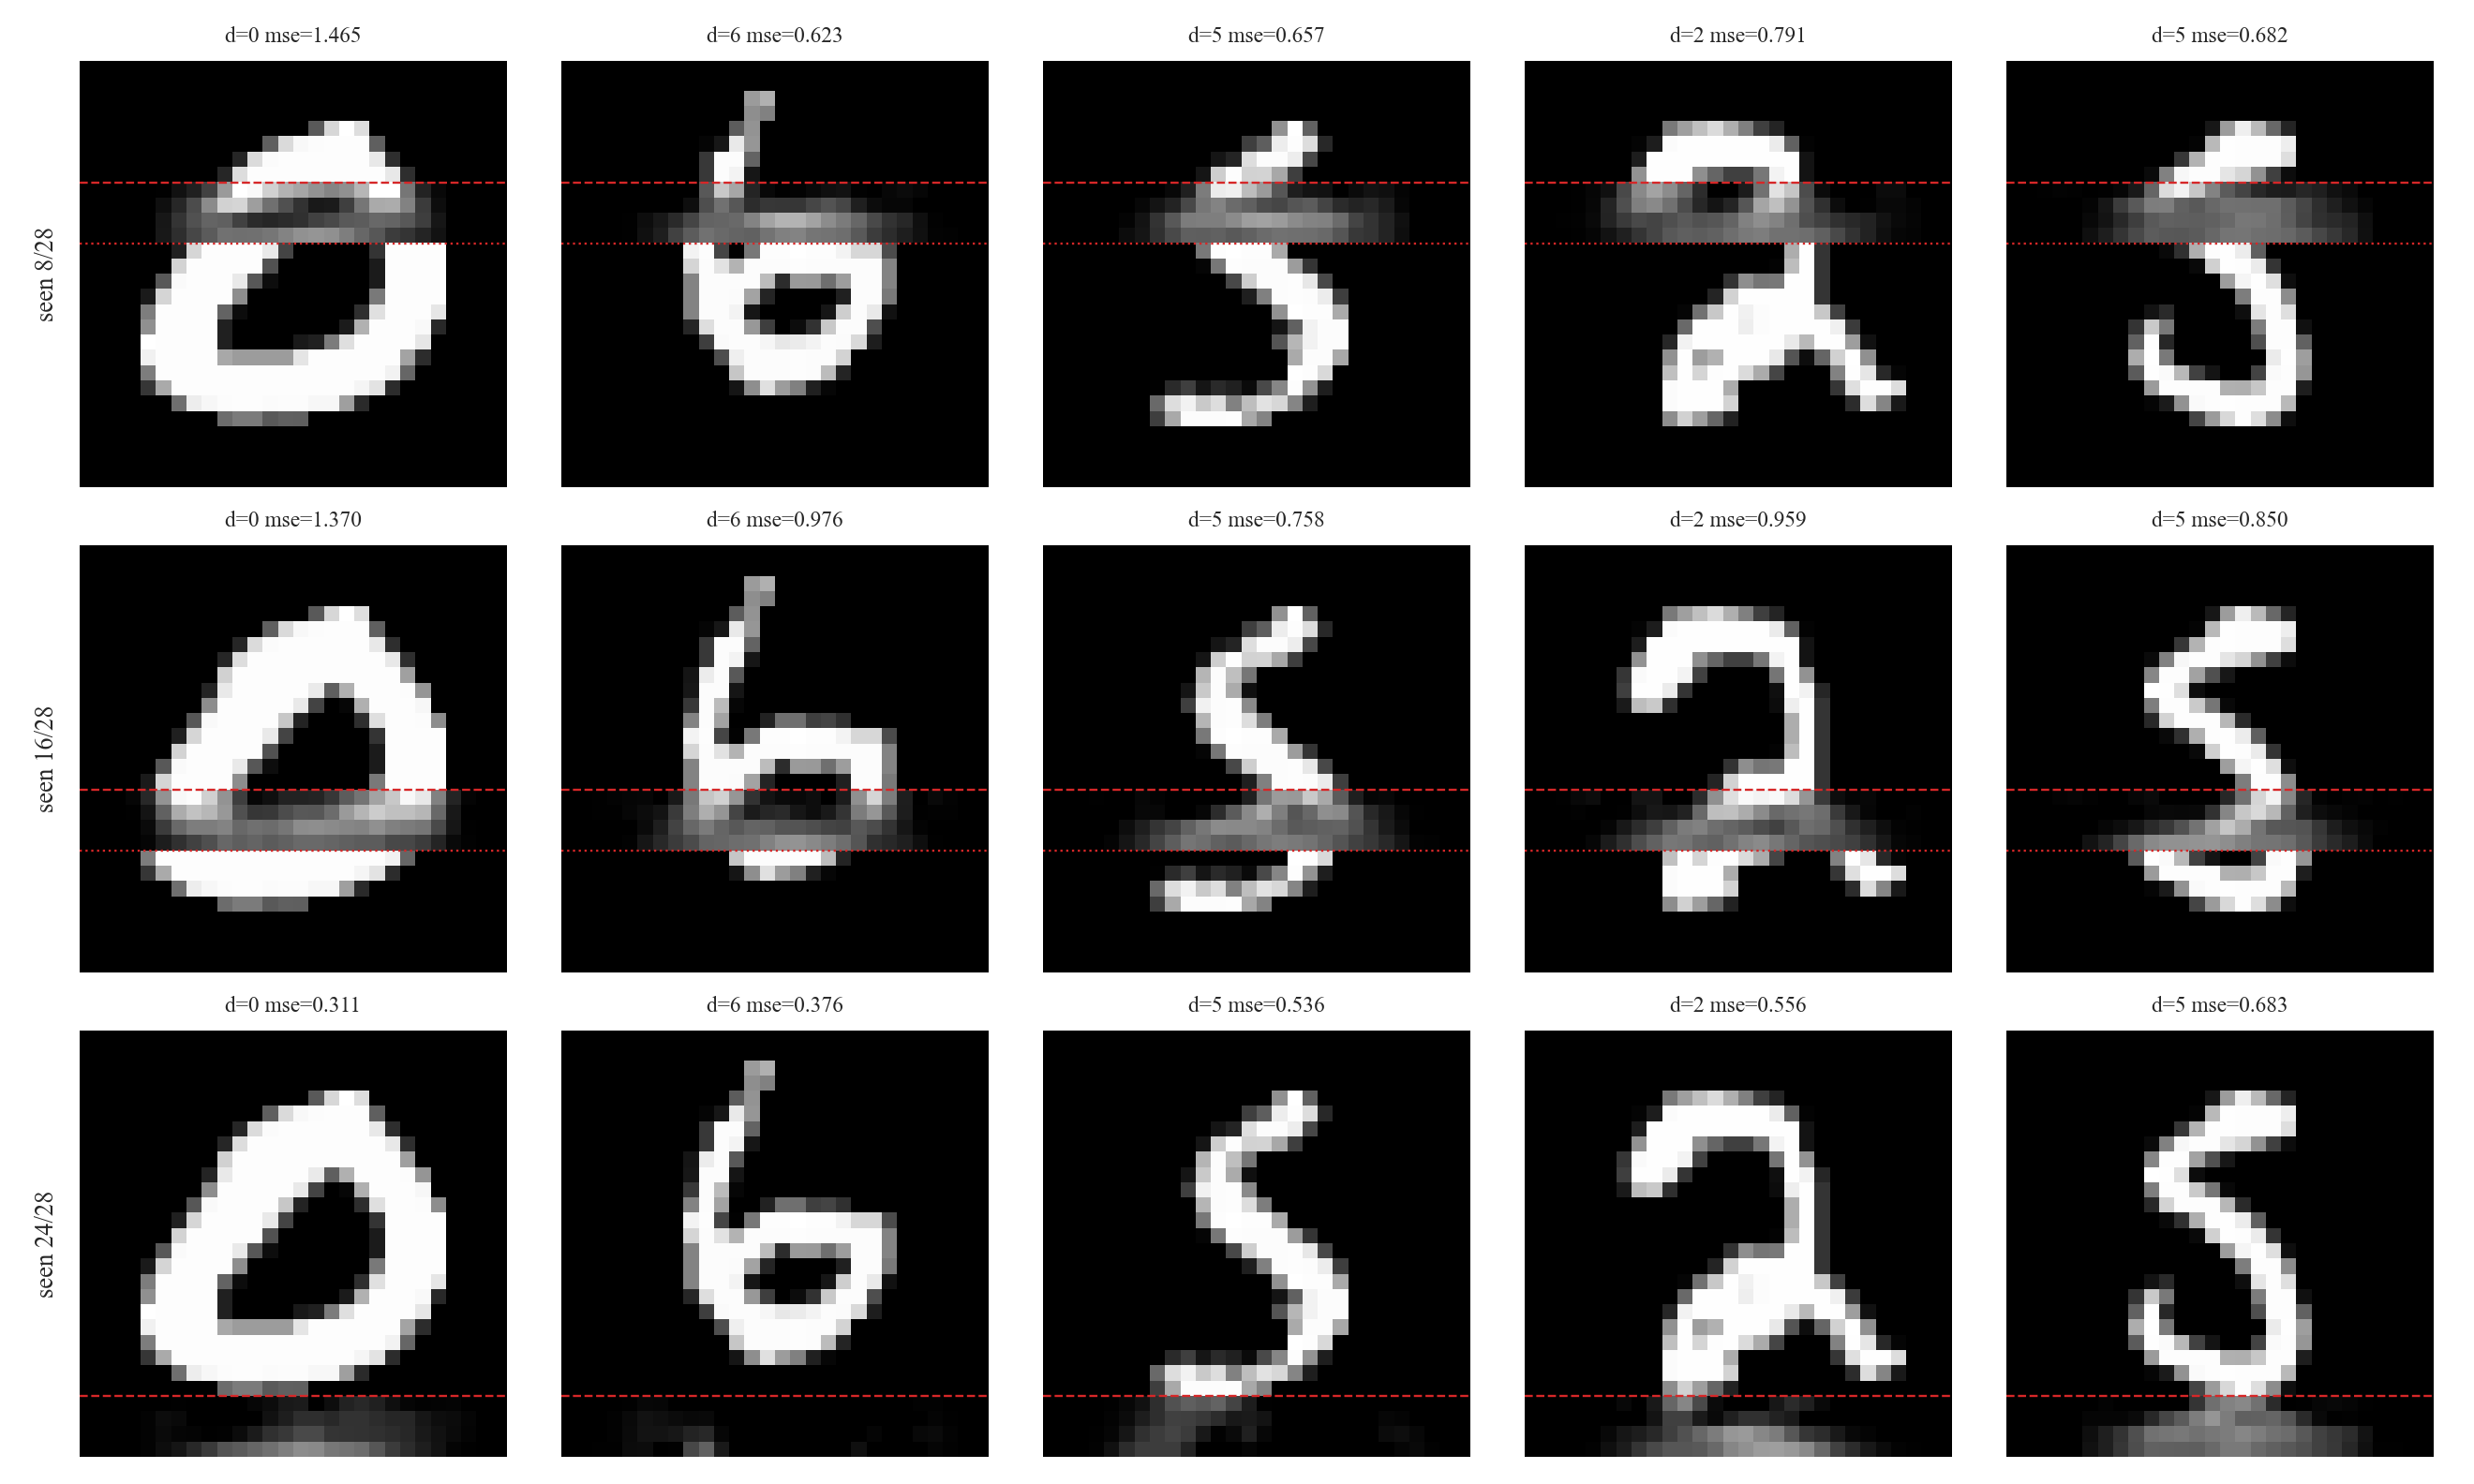
\includegraphics[width=0.49\linewidth]{terel_autoregressive_rows4_ctx_2_4_6of7.png}
  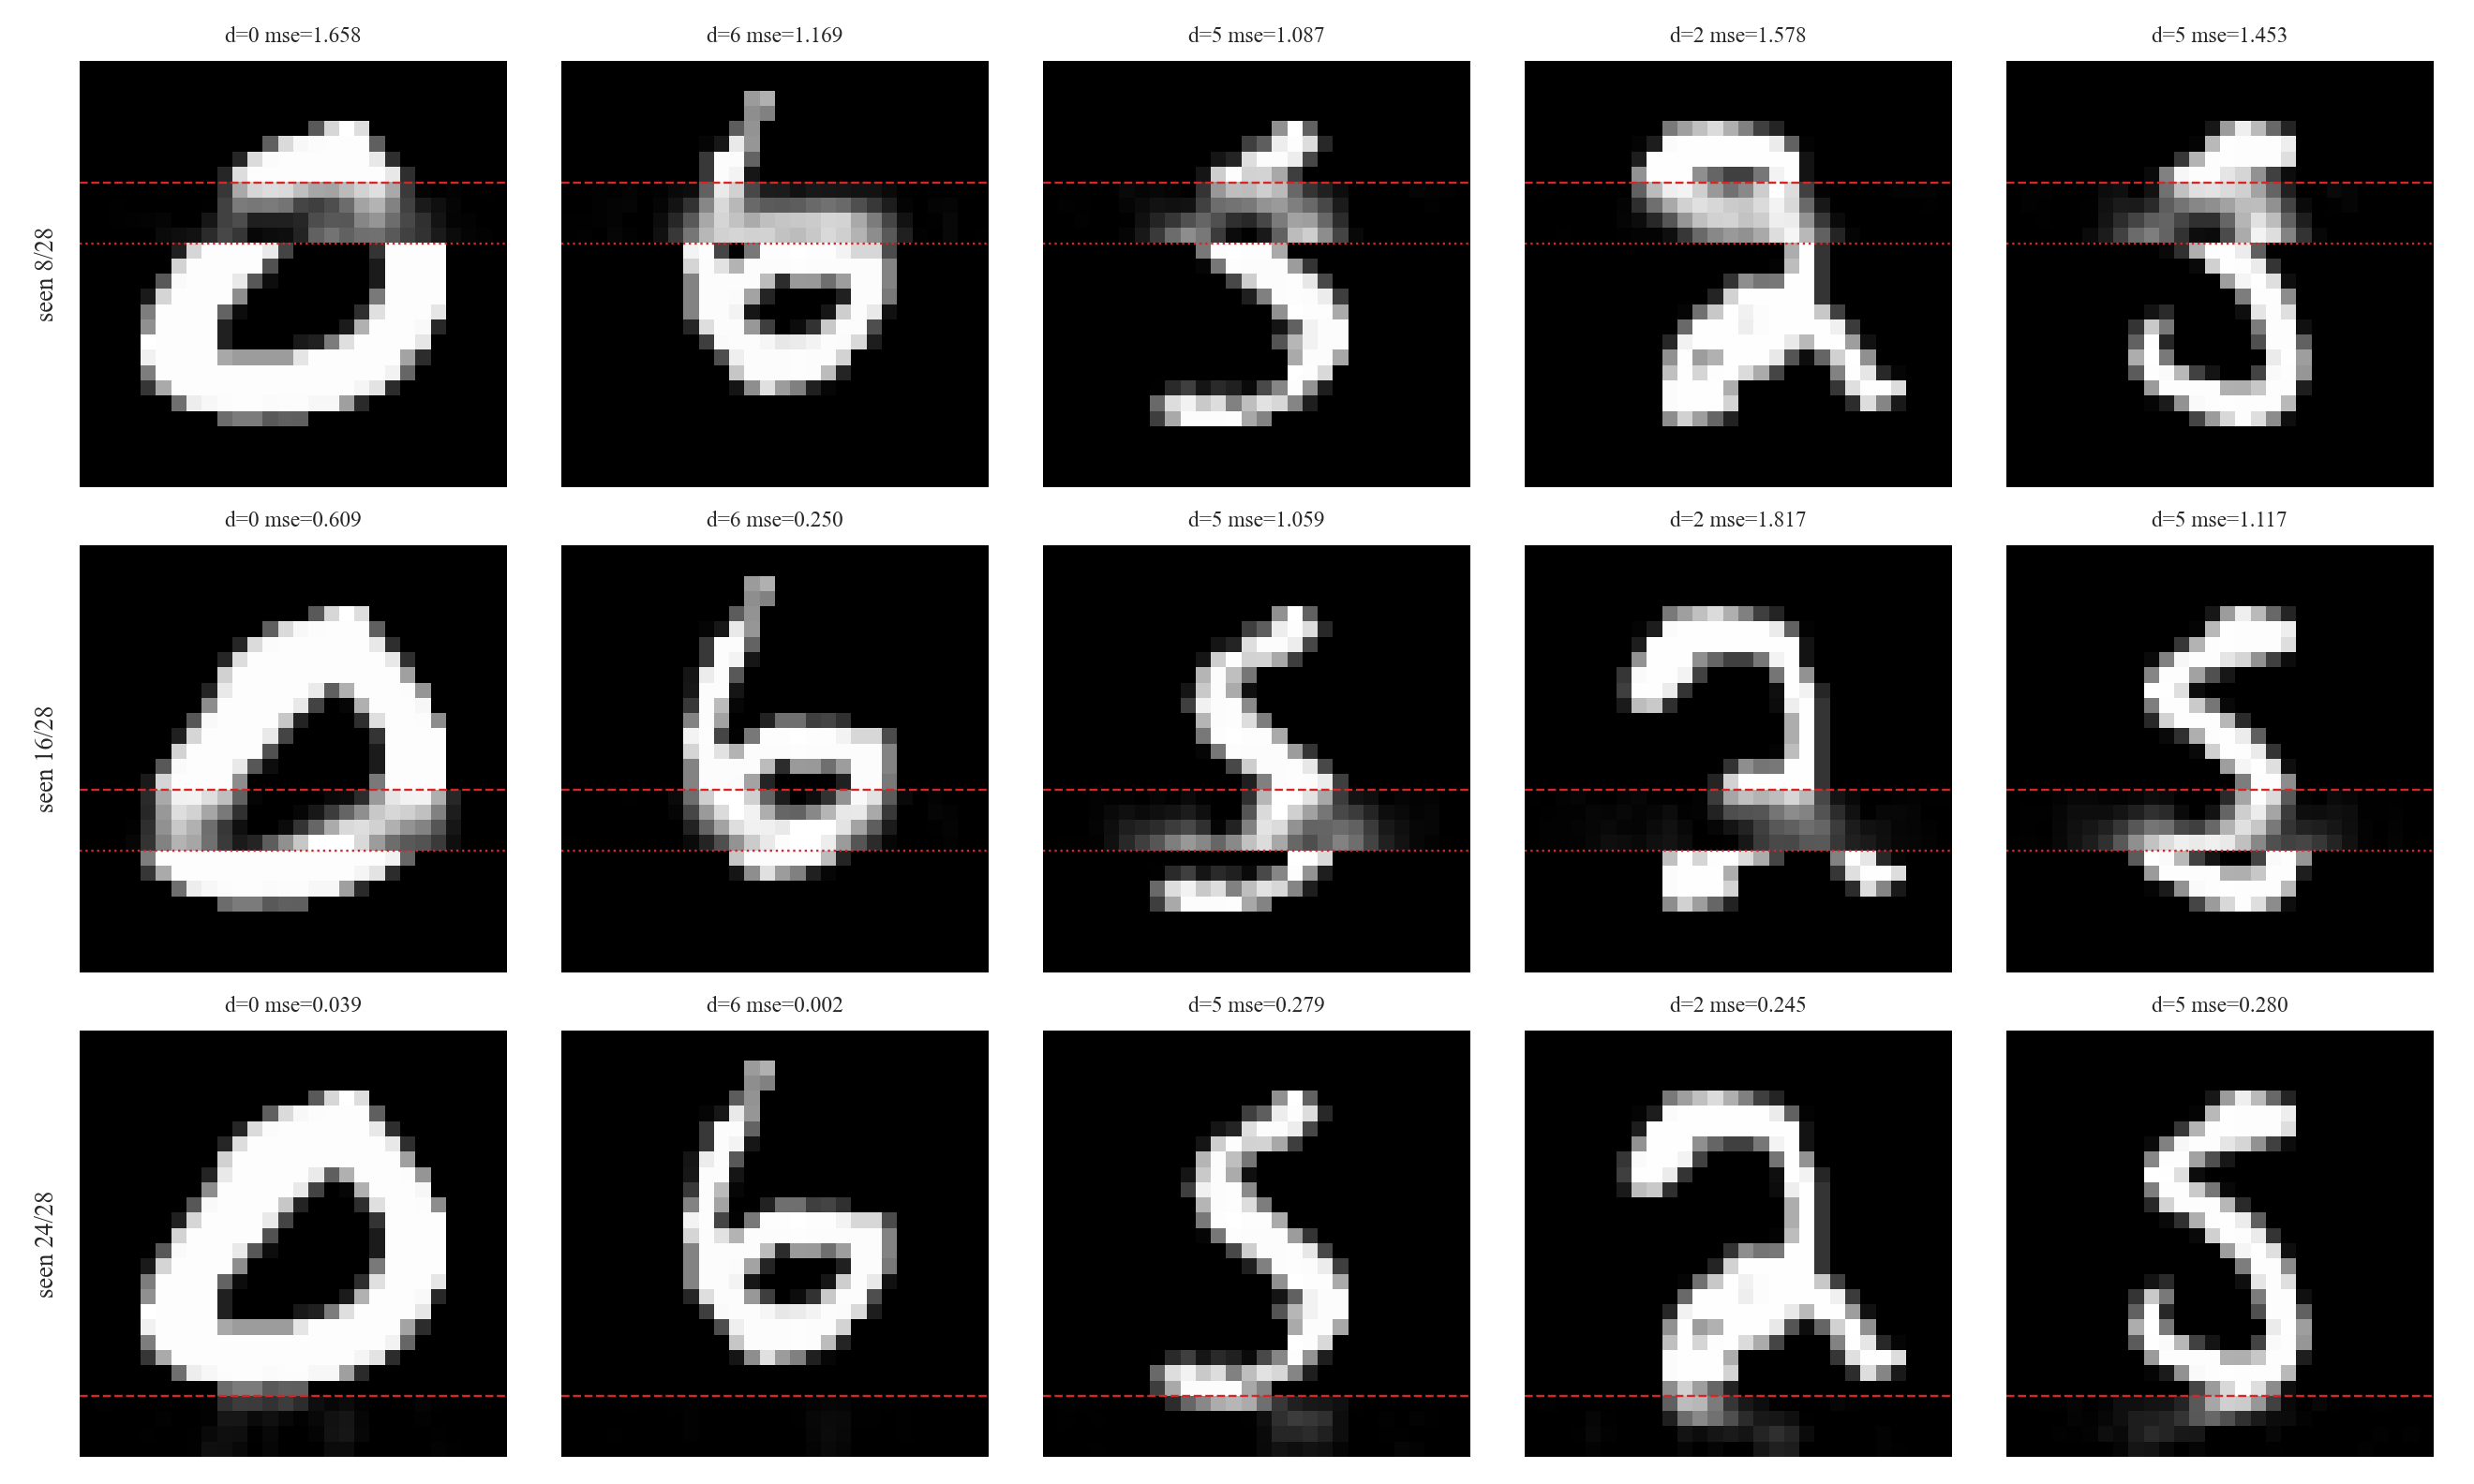
\includegraphics[width=0.49\linewidth]{bp_autoregressive_rows4_ctx_2_4_6of7.png}
  \caption{Autoregressive row completion on MNIST-Rows (left: TeReL, right: BP).}
  \label{fig:mnist_rows_rollout_rows4_ctx}
\end{figure}
\FloatBarrier

\noindent The TeReL setup used for these rollouts was trained concurrently. The exact repository state at the point of generation is recorded in the repository README.
